\hypertarget{quelques-jours-uxe0-kyushu}{%
\section{Quelques jours à Kyushu}\label{quelques-jours-uxe0-kyushu}}

En arrivant au Japon, nous nous sommes rendus compte que nous n'avions
pas de programme clair. La procédure de visa pour la Russie et la Chine
nous avait forcé à définir nos étapes avant de partir, donc nous sommes
arrivés un peu les mains dans les poches. Une fois passée l'euphorie de
retrouver mon pays de coeur et après un premier aperçu d'Osaka, nous
avons décidé de commencer notre séjour par l'île de Kyushu, l'île la
plus au sud de l'archipel nippon, que je ne connaissais pas du tout.

\begin{figure}
\centering
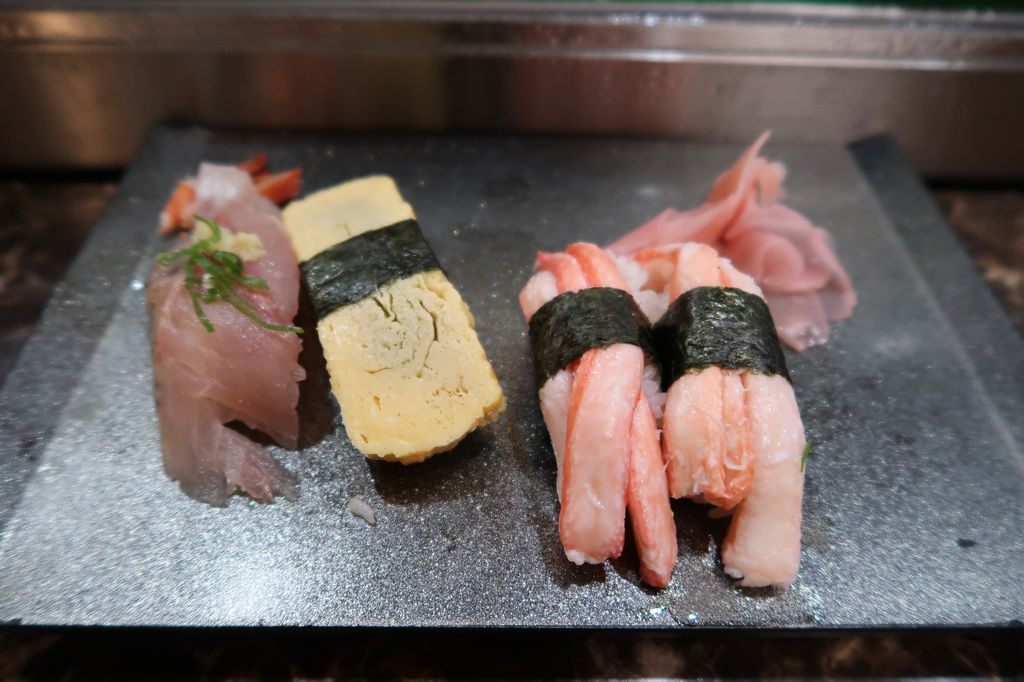
\includegraphics{images/20180709_sushi.JPG}
\caption{Après l'effort, le réconfort : de délicieux sushis mangés à
Osaka.}
\end{figure}

Au programme : la visite des villes de Fukuoka, Nagasaki et Kagoshima.
Nous avons pris nos quartiers à Fukuoka étant donné qu'avec
l'indispensable Japan Rail Pass on peut facilement (et économiquement)
prendre un train rapide vers les autres villes de l'île.

Fukuoka est la grande ville au nord de Kyushu. Nous avons profité des
conseils d'une expatriée et amoureuse du coin,
\href{http://www.benefukuoka.com/2015/12/fukuoka-conseils.html}{Béné no
Fukuoka}, pour découvrir les quartiers de cette ville découpée par des
canaux. La balade autour de la Fukuoka Tower a révélé une jolie plage
(depuis le temps qu'on avait pas mis les pieds dans le sable...) où les
poissons-volants offraient un drôle de spectacle au coucher du soleil.
Nous y avons mangé des \emph{Hakata ramen}, spécialité de pâtes
renommée, et y avons vu les préparatifs du festival Gion-Yamakasa. Il
s'agit d'une course de chars décorés de manière impressionnante,
opposant les différents quartiers de Fukuoka, portés à travers la ville
par des équipes d'hommes portant ce qui ressemble étrangement à des
"culottes" de sumo ; on vous laisse imaginer !

Nagasaki, c'est bien sûr la ville du drame atomique, mais aussi un port
de commerce qui a marqué l'histoire du Japon. Nous avons ainsi découvert
le complexe de Dejima, île artificielle installée en bordure de la ville
au 16ème siècle pour accueillir les portugais et hollandais de passage
(et circonscire fermement leur influence). L'île avait disparu avec le
temps, englobée par l'extension de Nagasaki, mais des fouilles ont
permis de la reconstituer avec un extraordinaire sens du détail. Quant
au musée de la bombe, il permet de se rendre compte de la gravité et de
l'horreur de l'évènement. Le parc de la paix, à côté, souligne le
message du musée de manière paisible.

\begin{figure}
\centering
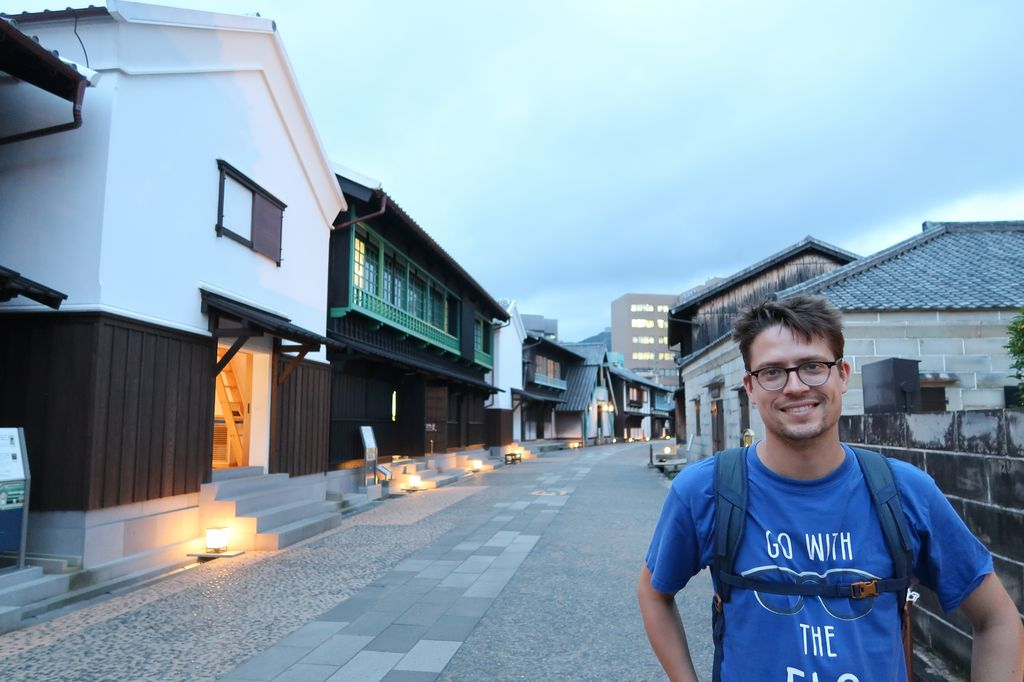
\includegraphics{images/20180709_dejima.JPG}
\caption{On peut vraiment passer des heures sur l'île reconstituée de
Dejima.}
\end{figure}

Enfin, Kagoshima. Une ville célèbre pour son rapport à l'île volcanique
avoisinante, Sakurajima. Peut-on vivre à côté d'un double-volcan avec
deux éruptions majeures au 20ème siècle à son actif, et qui crache des
cendres de façon quotidienne ? Il semblerait que oui. Les habitants vont
même jusqu'à collecter les cendres dans les sacs en plastique mis à
disposition par la ville (et que les touristes peuvent acheter
\^{}\^{}). Malheureusement, Sakurajima a gardé la tête dans les nuages
pendant notre journée à l'arpenter. L'île est un bel endroit pour
marcher et acheter des légumes, car le sol y est très fertile. On y a
d'ailleurs déjà fait pousser un radis de 30 kilogrammes...

\begin{figure}
\centering
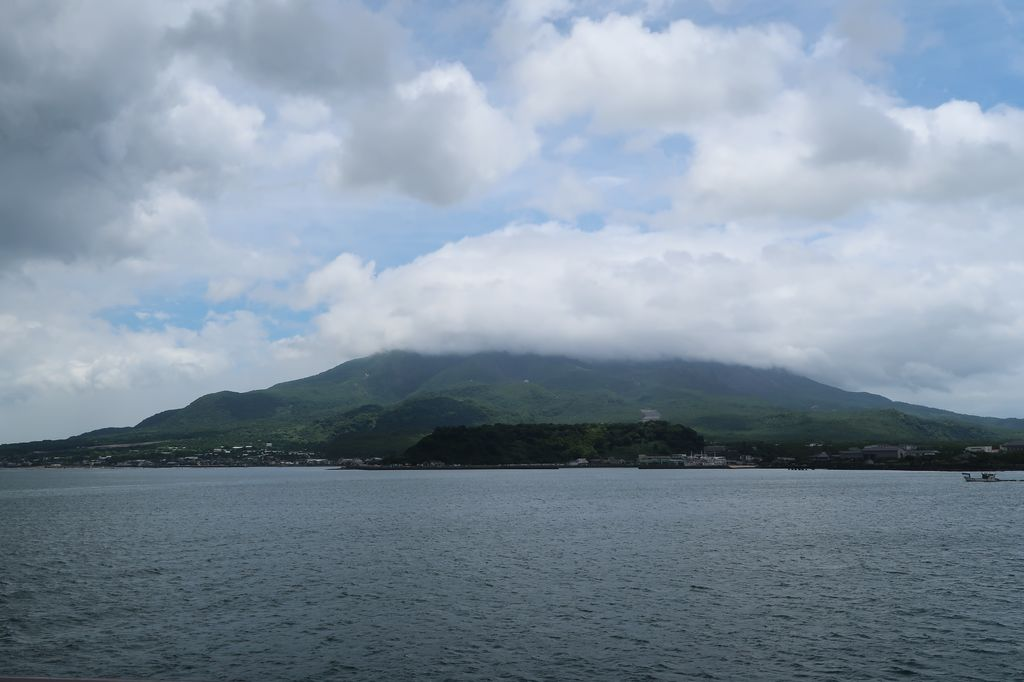
\includegraphics{images/20180709_sakurajima.JPG}
\caption{Île volcanique à l'horizon, capitaine !}
\end{figure}

Et voilà le récit de nos premiers jours au Japon, on vous laisse
maintenant découvrir les photos ci-dessous !

\emph{Florian et Elida}
